

\documentclass[letterpaper, 10 pt, conference]{ieeeconf}  % Comment this line out if you need a4paper

%\documentclass[a4paper, 10pt, conference]{ieeeconf}      % Use this line for a4 paper

\IEEEoverridecommandlockouts                              % This command is only needed if 
                                                          % you want to use the \thanks command

\overrideIEEEmargins                                      % Needed to meet printer requirements.

% See the \addtolength command later in the file to balance the column lengths
% on the last page of the document

% The following packages can be found on http:\\www.ctan.org
%\usepackage{graphics} % for pdf, bitmapped graphics files
%\usepackage{epsfig} % for postscript graphics files
%\usepackage{mathptmx} % assumes new font selection scheme installed
%\usepackage{times} % assumes new font selection scheme installed
%\usepackage{amsmath} % assumes amsmath package installed
%\usepackage{amssymb}  % assumes amsmath package installed
\usepackage{cite}
\usepackage{mathtools}
\usepackage{cleveref}


\title{\LARGE \bf
Magnetic Hammer Actuation for Tissue Penetration using Millirobots
}


\author{Julien Leclerc, Ashwin Ramakrishnan, Nikolaos V. Tsekos and Aaron T. Becker % <-this % stops a space
\thanks{This work was supported by the National Science Foundation, Grant No. 1646566. }% <-this % stops a space
\thanks{Authors are with the Dept. of Electrical and Computer
Engineering, University of Houston, Houston, TX 70004, USA
        {\tt\small jleclerc@uh.edu}}%
%\thanks{$^{2}$Bernard D. Researcheris with the Department of Electrical Engineering, Wright State University,
%       Dayton, OH 45435, USA
%      {\tt\small b.d.researcher@ieee.org}}%
}


\begin{document}



\maketitle
\thispagestyle{empty}
\pagestyle{empty}


%%%%%%%%%%%%%%%%%%%%%%%%%%%%%%%%%%%%%%%%%%%%%%%%%%%%%%%%%%%%%%%%%%%%%%%%%%%%%%%%
\begin{abstract}

Untethered navigation of millirobots within a human body using an MRI scanner is a promising technology for minimally invasive surgery or drug delivery. However, the magnetic field and gradient values are too small to produce forces large enough to penetrate tissue. This paper presents a method to produce large pulsed forces on millirobots. A ferromagnetic sphere is placed inside the robot body and can move back and forth. This movement is created by alternatively changing the magnetic gradient direction. On the posterior side, a spring allows the sphere to change direction smoothly. On the forward side, a hard rod creates a surface for the sphere to impact. This impact results in a large pulsed force. This system has first been modeled and simulated. Different control strategies are presented and experimentally tested. Finally, the system was tested to penetrate artificial tissues. 

\end{abstract}


%%%%%%%%%%%%%%%%%%%%%%%%%%%%%%%%%%%%%%%%%%%%%%%%%%%%%%%%%%%%%%%%%%%%%%%%%%%%%%%%
\section{INTRODUCTION}

The navigation of millimeter-scale robots through the passageways of bodies is currently being studied as a method to perform highly localized drug delivery or perform minimally invasive surgery \cite{7067029,702,mi2020295}. Untethered navigation can be achieved by placing a ferromagnetic piece inside the robot and producing a controlled magnetic field around a patient. Propulsion and steering of millirobots can be accomplished by either moving a permanent magnet assembly around a patient \cite{taylor} or by controlling the current inside electromagnets \cite{MRM21638}. The latest solution is often realized with an MRI scanner which already includes several electromagnets. In that case, the background field magnetizes the ferrous piece of the robot, and the gradients coils produce the magnetic gradient necessary to produce forces. The MRI scanner can be used simultaneously to provide real-time imaging of the operating area as well as positioning of the robots.\par
The value of the forces generated on the millirobots is proportional to the field gradient strength. Commercial MRI scanner produces gradients in the range of 20 to 40 mT/m. This value could allow the navigation of robots through the body fluids but not the penetration of tissues. Tissue penetration indeed requires larger forces \cite{7139341}. This paper presents a method that allows producing large pulsed forces for tissue penetration. This system has been called magnetic hammer.\par
The magnetic hammer is a system embedded into the millirobot. The millirobot has a tubular structure in which a ferromagnetic sphere can move back and forth. This movement is produced by alternatively changing the gradient direction. On the posterior side of the millirobot, a spring allows the sphere to change direction with minimal energy loss. On the forward side, a hard rod creates a surface for the sphere to impact (impact plate). Repeated impacts result in large pulsed forces that allow penetrating body tissues progressively. 
A magnetic test bench has been developed to make experimental tests more practical and less expensive. It includes coils, sensors, power electronics and a real-time controller. Analytical models and numerical simulations have been validated with the experimental results, for different cases.\par

\begin{figure}
  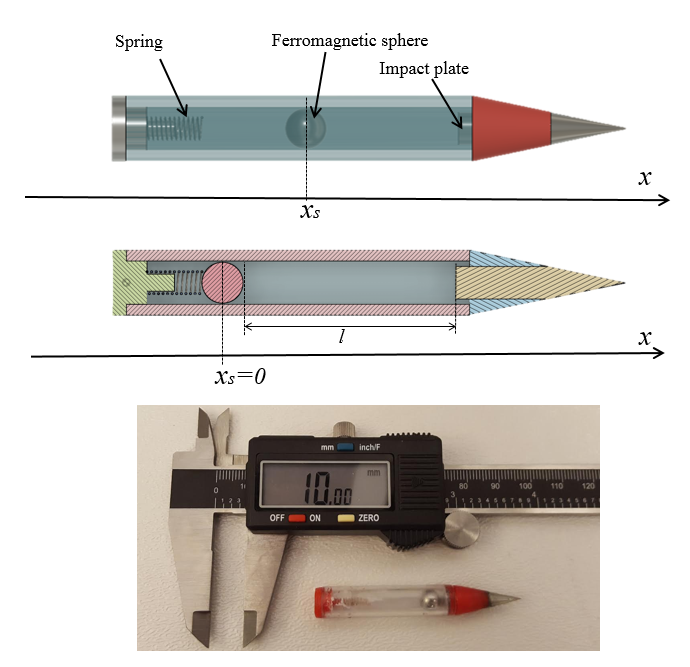
\includegraphics[width=\linewidth]{figure1-2.png}
  \caption{schematic representation of a millirobot actuated by a magnetic hammer}
  \label{millirobot}
\end{figure}

\begin{figure}
	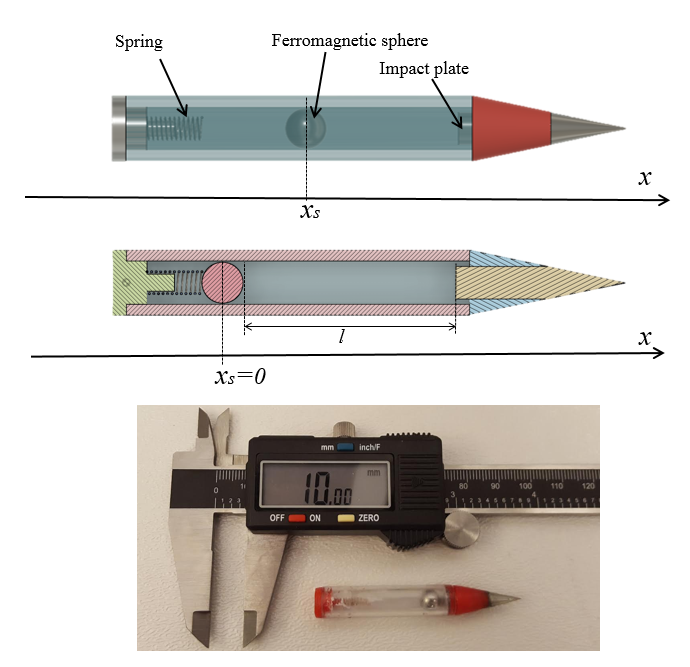
\includegraphics[width=\linewidth]{figure1-2.png}
	\caption{schematic representation of a millirobot actuated by a magnetic hammer}
	\label{millirobot}
\end{figure}

The paper is organized as follow: first, the system is mathematically modeled, and its behavior is studied. Secondly, the parameters of the model are experimentally measured. Different materials for the impact plate are compared. Thirdly, the magnetic test bench is described, and different control methods are tested (open loop, partially closed loop, and closed loop). Results are compared to the mathematical model. Finally, the system is tested to penetrate artificial tissues made with agar. The last section is a conclusion of this study.


\section{Theoretical study}

\subsection{Mechanical model}
The motion of the sphere between two consecutive impacts can be divided into 4 different phases, based on the forces that act on it. The magnetic gradient force $F_mag$ and friction force $F_f$ act on the sphere during its motion along the free length of the tube (See Fig. 2a,d). When the spring is compressed, its reaction force $F_s$ acts on the ball as well(See Fig. 2 b,c). $F_mag$  

\begin{figure}
	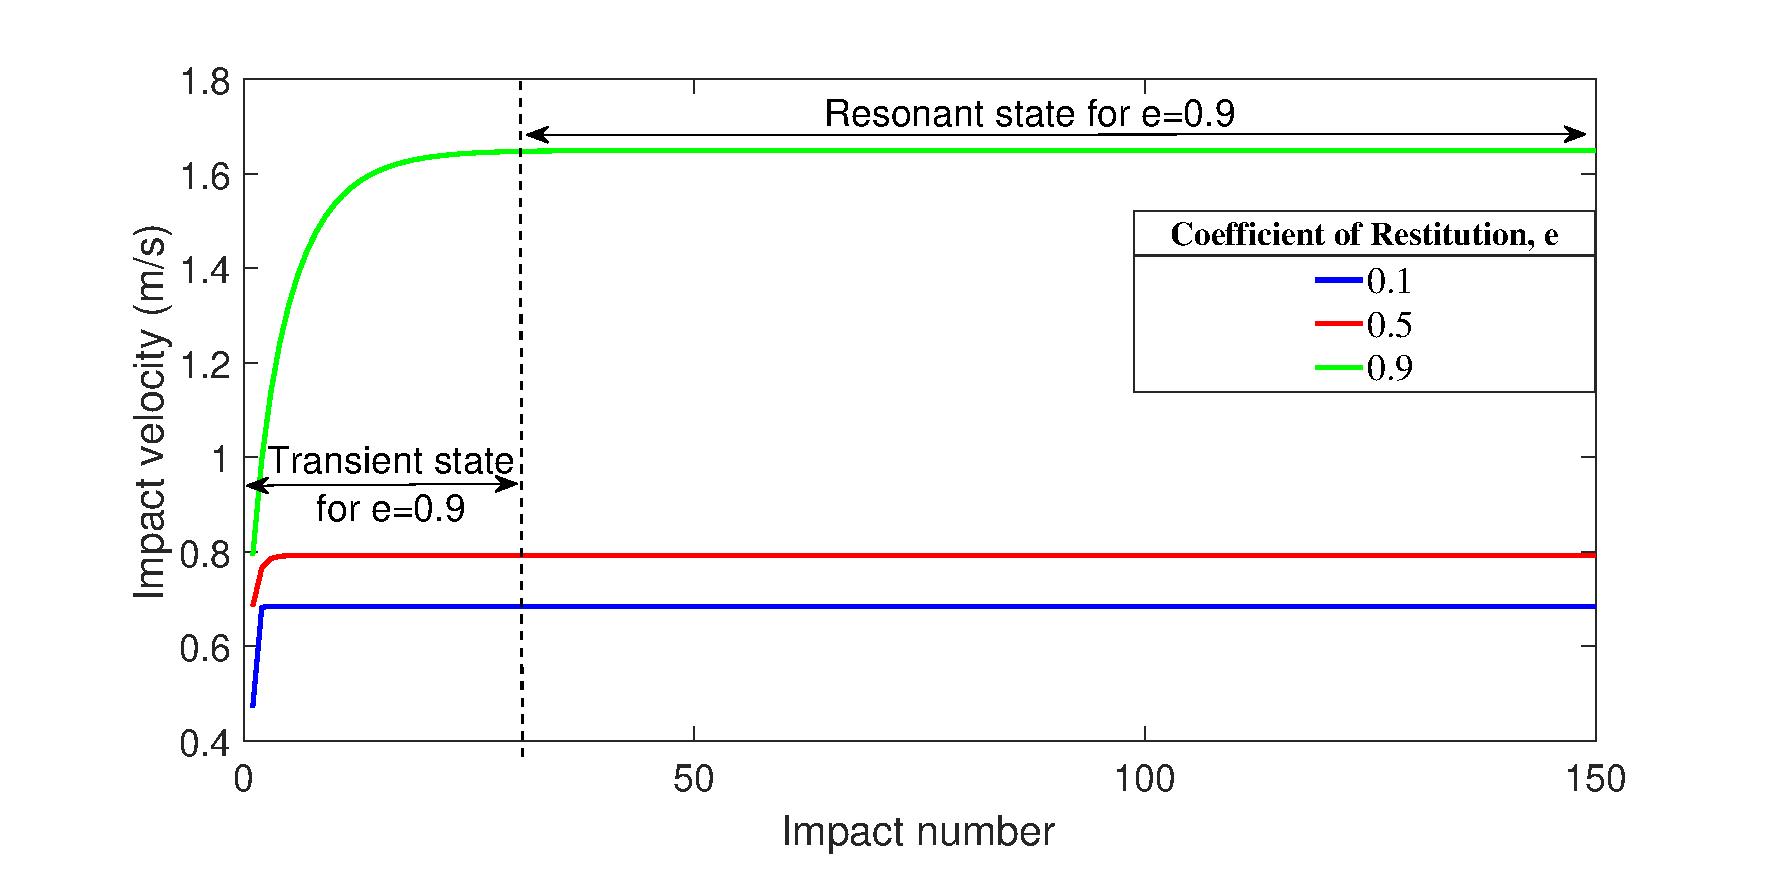
\includegraphics[width=\linewidth]{Closedloop_Impact_velocity.eps}
	\caption{Closed loop impact velocity for 50 contacts}
	\label{Closedloop_Impact_velocity}
\end{figure}


\subsection{Magnetic field calculation}

The magnetic field generated by an MRI scanner can be separated into two components. The first is a constant, strong and uniform magnetic field $B_0$. This field is used to align the magnetic moments of the protons. Commercial MRI scanners have $B_0$ typically ranging from 1.5 to 3 T. The second component of the field is the magnetic gradient. It is used to encode the MRI signal spatially. The flux density $\mathbf{G}$ produced by the gradient coils is superposed to $B_0$ and linearly varies with position. A computer controls its value.\par
The modelisation of the field inside the uniformity sphere of an MRI scanner is straightforward. It is the sum of $B_0$ and $\mathbf{G}$. $\mathbf{G}$ is directly proportional to the current inside the gradient coils.

\begin{equation}
\mathbf{B}=\mathbf{B_0}+\mathbf{G},~~~
\mathbf{B_0}=\begin{bmatrix}
0\\ 
0\\ 
B_0
\end{bmatrix},~
\mathbf{G}=\begin{bmatrix}
k_x.I_x\\ 
k_y.I_y\\ 
k_z.I_z
\end{bmatrix}
\end{equation}

where $k_x$, $k_y$ and $k_z$ are the coils constants and $I_x$, $I_y$ and $I_z$ are the electrical current values.\par

The flux density is more complicated to calculate outside of the uniformity sphere. The same problem is present in our desktop experiment because the flux density and gradient are not constant. It is paramount to accurately compute the magnetic field to be able to calculate forces accurately. A method to calculate the field produced in all space by a solenoid assembly was used. It was tested on our desktop size experiment.\par
According to [], the magnetic flux density produced by a current loop in all space can be calculated using equations \cref{Bz1loop,Bteta1loop,delta,beta,single_loop_geometry}.
\begin{equation}
B_z=\frac{\mu _0.I}{2.\pi.\delta ^{2}.\beta  }\left [ \left ( a^2-\rho ^2-z^2 \right )(E(k^2)+\delta ^2.K(k^2)) \right ] 
\label{Bz1loop}
\end{equation}
\begin{equation}
B_\theta=\frac{\mu _0.I.z}{2.\pi.\delta ^{2}.\beta.\rho   }\left [ \left ( a^2-\rho ^2-z^2 \right )(E(k^2)-\delta ^2.K(k^2)) \right ]
\label{Bteta1loop}
\end{equation}
\begin{equation}
\delta =\sqrt{a^2+R_m^2+Z_m^2-2.a.R_m}
\label{delta}
\end{equation}
\begin{equation}
\beta =\sqrt{a^2+R_m^2+Z_m^2+2.a.R_m}
\label{beta}
\end{equation}

\begin{figure}
  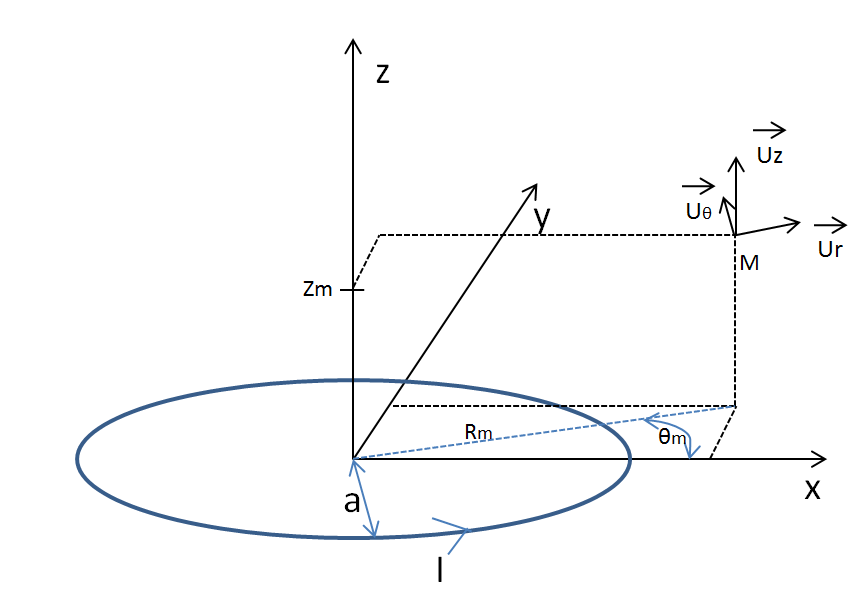
\includegraphics[width=\linewidth]{single_loop.png}
  \caption{Geometry and variables used in equation \cref{Bz1loop,Bteta1loop,delta,beta}}
  \label{single_loop_geometry}
\end{figure}

The cross-section $S$ of any solenoid can be divided into infinitesimal sections $dS$. Each $dS$ is subjected to a current $dI=J.dS$. This current $dI$ forms an infinitesimal loop, and the field it produces can be calculated using \cref{Bz1loop,Bteta1loop,delta,beta}. By integrating this equation over the solenoid cross-section, one can obtain the value of the flux density generated by the solenoid.\par
The flux density has to be calculated for each solenoid. The total flux density is the vectorial sum of the flux density produced by each solenoid.

\begin{figure}
  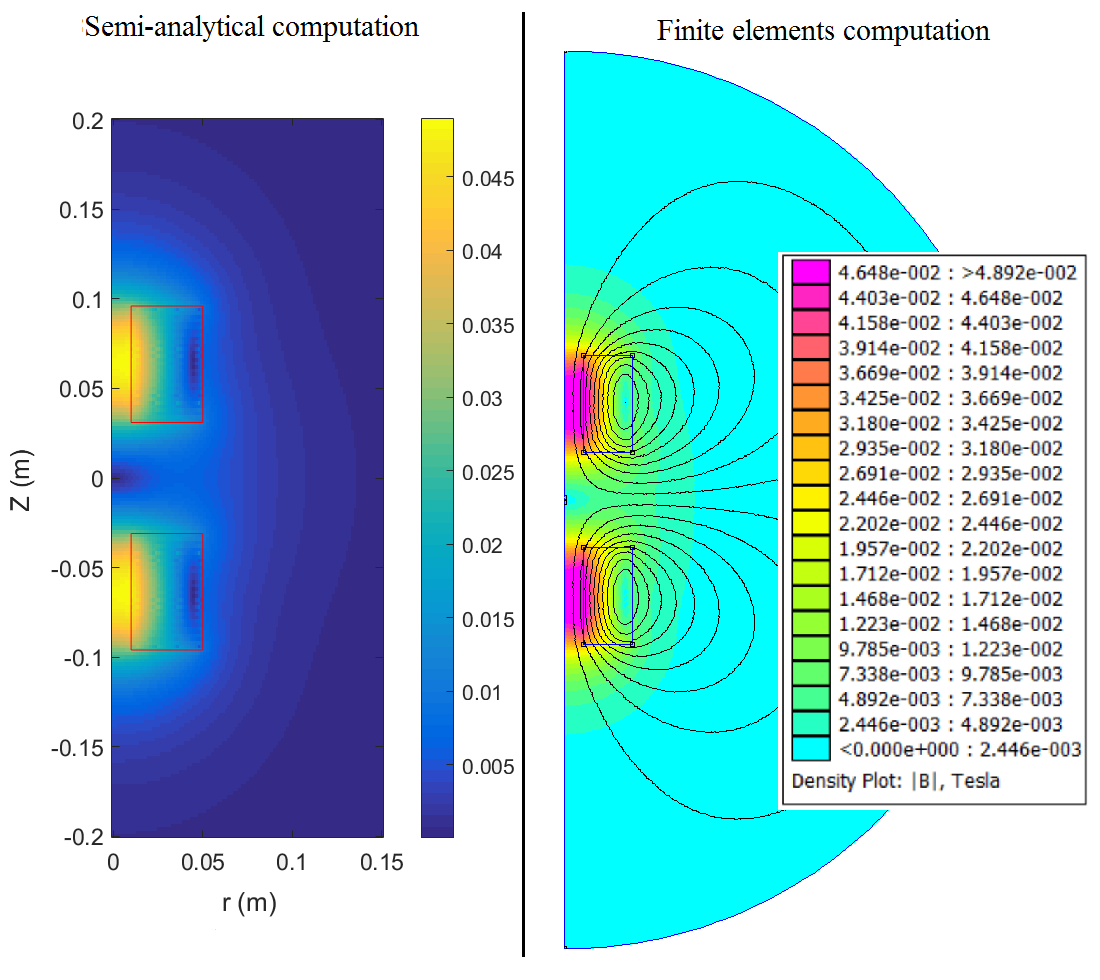
\includegraphics[width=\linewidth]{Femm_matlab_comparison.png}
  \caption{Comparison between the flux density computed the semi-analytical method with Matlab and the flux density computed via a finite elements method with FEMM.}
  \label{Femm_matlab_comparison}
\end{figure}

\subsection{Magnetic force calculation}

This section aims at calculating the force applied by the magnetic field to the sphere.\par
The ferromagnetic sphere is small compared to the coil system and can be considered as a punctual infinitely small magnetic moment $\mathbf{m}$. Assuming a constant material magnetization $M$, one can calculate $m$ from \ref{mag}. $V$ is the volume of the sphere.
The ferromagnetic sphere is magnetized by the externally applied field $H_{app}=B_{app}/\mu_0$. Ferromagnetic materials create a demagnetizing field $Hd$ when subjected to an external field. The actual field $H$ seen by the sphere is the sum of $Happ$ and $Hd$. This effect has to be taken into account to calculate the magnetization accurately. $Hd$ is related to $H_{app}$ by \ref{hd}. The demagnetization factor $N$ for a sphere is -1/3. Its magnetization can be calculated using \ref{mag2}.
Once the magnetic moment $m$ is obtained, the force on the sphere can be calculated using \ref{force}.

\begin{equation}
\mathbf{m}=\mathbf{M}.V
\label{mag}
\end{equation}

\begin{equation}
\mathbf{H_d}=N.\mathbf{H_{app}}
\label{hd}
\end{equation}

\begin{equation}
\mathbf{M}=\frac{\mathbf{H_{app}}\left ( \mu_r-1  \right )}{2.N.\mu_r-1}
\label{mag2}
\end{equation}

\begin{equation}
\mathbf{F}=\mathbf{\nabla}(\mathbf{m}.\mathbf{B})
\label{force}
\end{equation}

\subsection{Simulation results}

\begin{figure}
  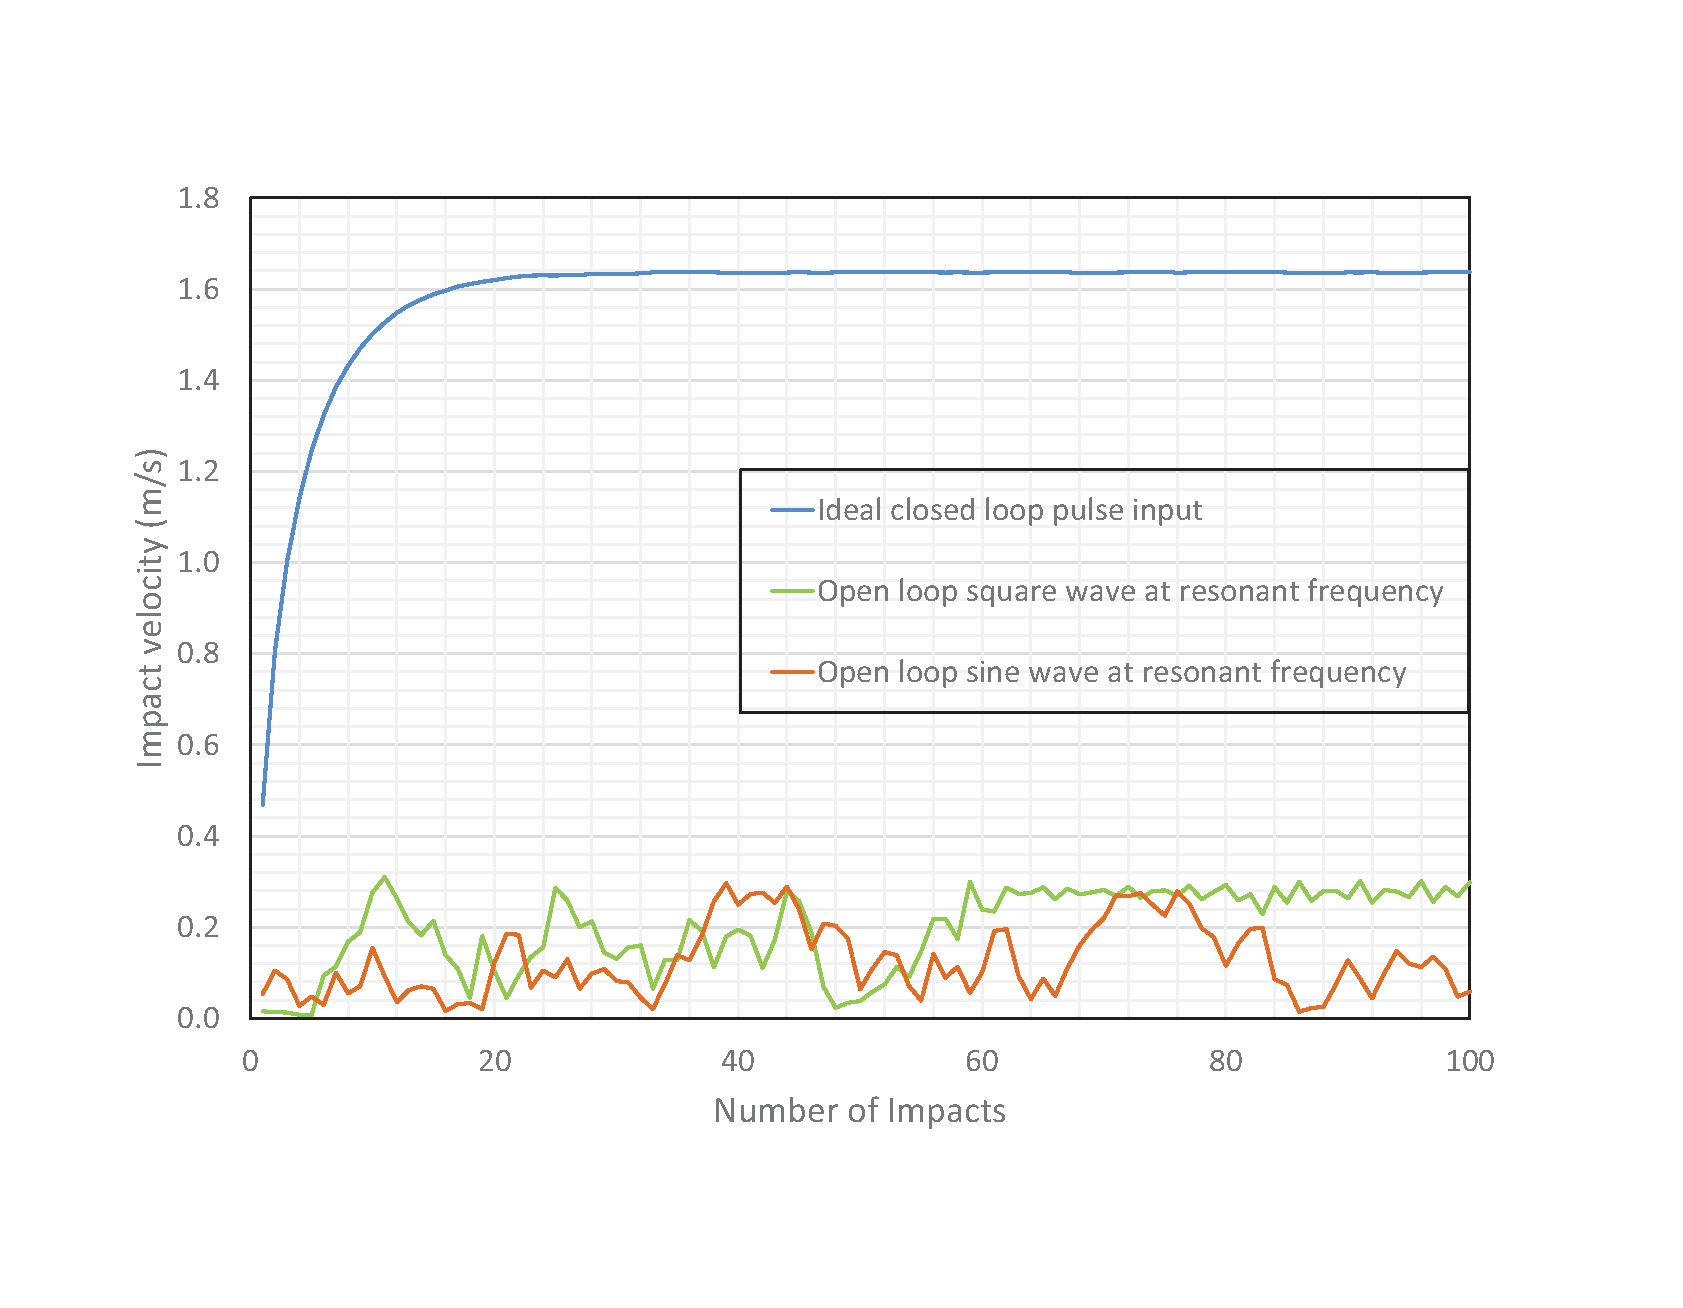
\includegraphics[width=\columnwidth,scale=1]{close_vs_openloop.eps}
  \caption{Geometry and variables used in equation \cref{Bz1loop,Bteta1loop,delta,beta}}
  \label{close_vs_open_loop}
\end{figure}

\begin{figure}
	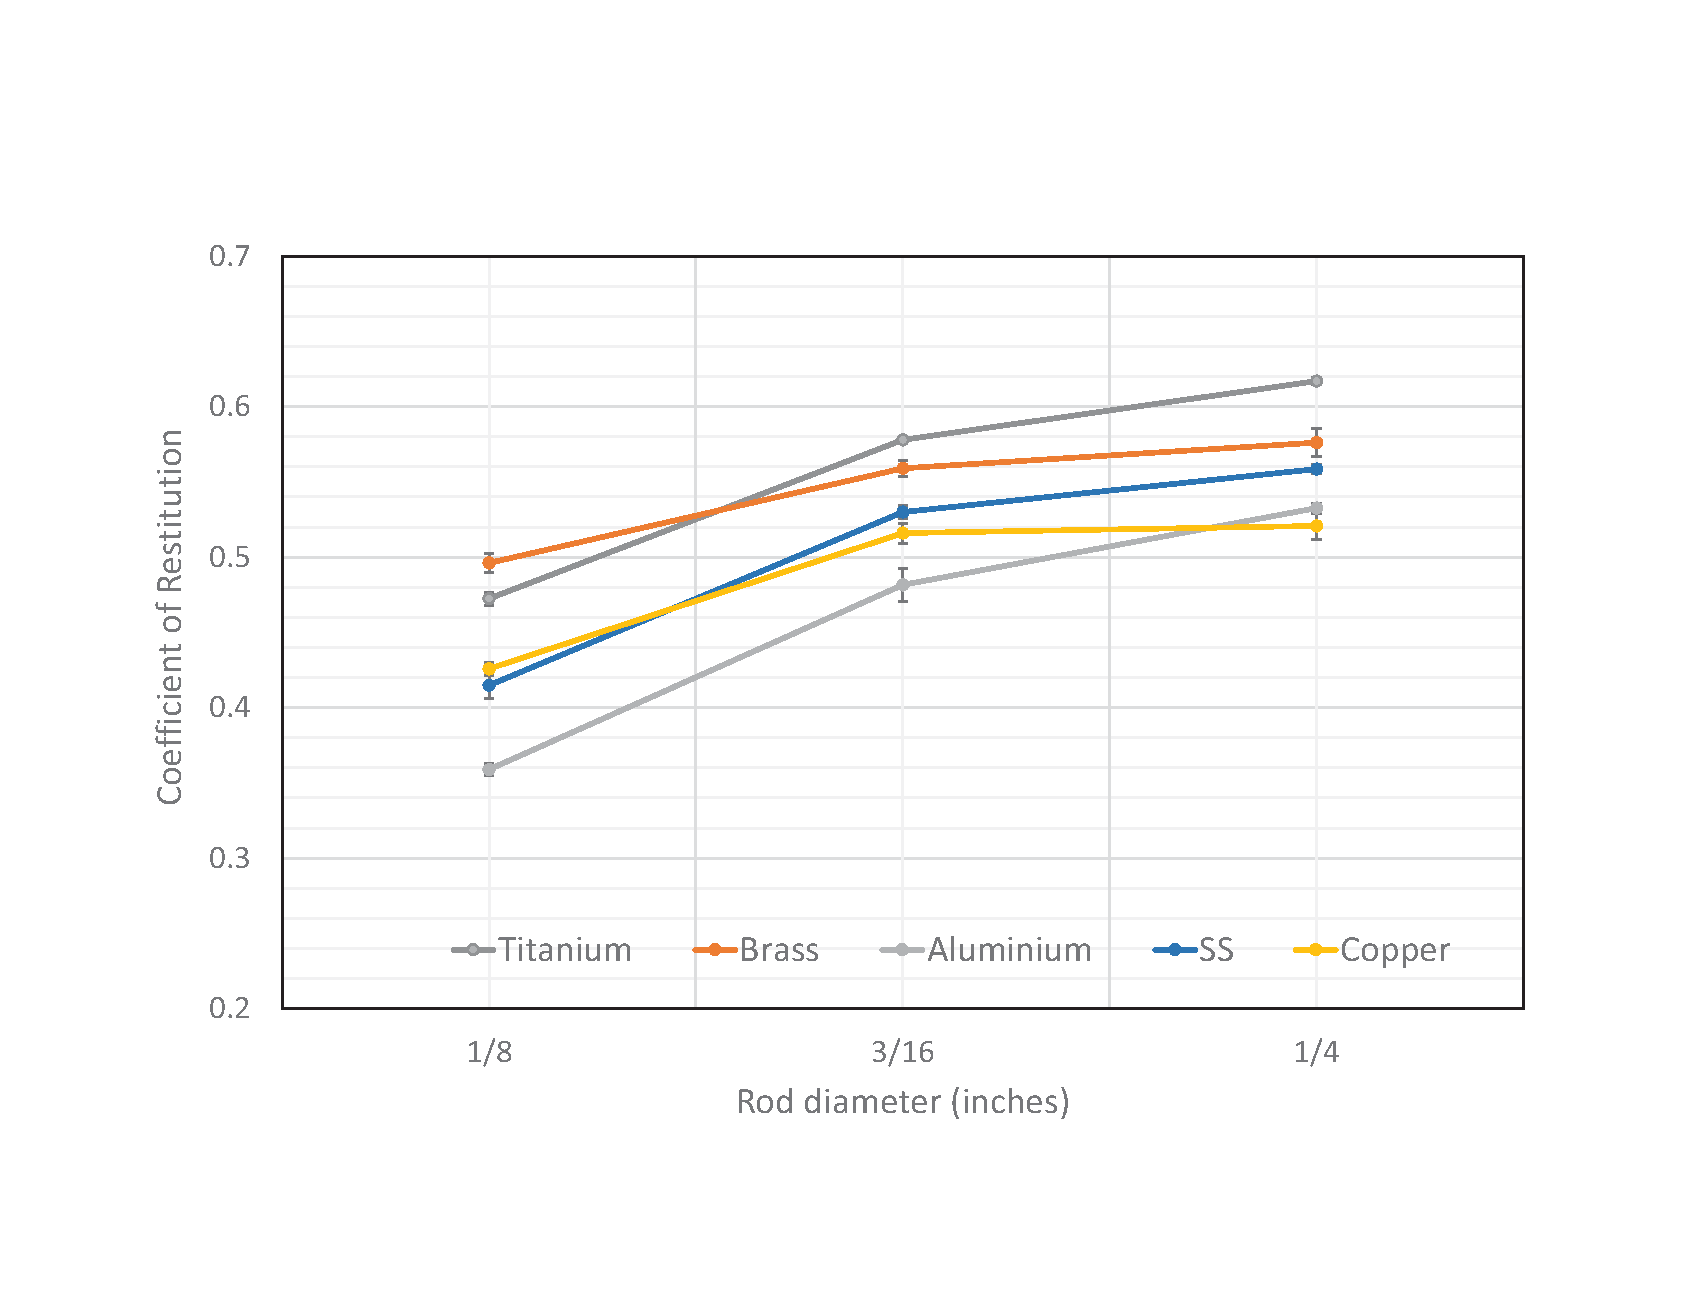
\includegraphics[width=\linewidth]{CoR_measurements.eps}
	\caption{CoR values for different materials}
	\label{CoR_measurements}
\end{figure}

\section{Experimental determination of model parameters}

\subsection{Impact coefficient of resititution}


The coefficient of restitution '$e$' was determined using the time interval between two consecutive bounces of the sphere when dropped from a given height, onto the impact rod. The measurements were made using 1" long impact rods for five different materials. As seen in figure \ref{fig:CoR_setup_data}

\begin{figure}
	\includegraphics[width=\columnwidth]{CoR_setup_data.eps}
	\caption{Experimental setup for measuring CoR}
	\label{CoR_setup_data}
\end{figure}


\subsection{Frictional coefficient}

This subsection has not been proofread.

The friction between the moving sphere and the other components of the millirobot was included into the model. The sphere can be rolling or sliding inside the tube. The modelization is based on the method described in []. 
The friction on the tube produces a torque on the sphere. It is assumed that the coefficient of static friction is equal to the coefficient of kinetic friction. The equation used to calculate the angular velocity vaiartion of the sphere is different wether the sphere is rolling or sliding. The distinction between these two different behavoiur is made by calculating the relative velocities of the sphere and the tube surface (see eq?). \par
If the relative speed is inferior to 0.005 m/s and if the force applied to the sphere is smaller than the kinetic friction, the sphere is considered to be rolling inside the tube and the drag is null. domega/dt can be calculated with:
In all other cases, the torque applied to the sphere is equal to the kinetic friction force multiplied by the sphere radius. The drag is equal to the kinetic friction force.


\section{Experimental magnetic hammer tests}

\subsection{Magnetic test bench description}

A desktop-size single axis magnetic setup was built to reduce the cost related to clinical MRI experiments. It is composed of two solenoid coils oriented along the same axis and separated by a distance $d$. The coils are used to produce both the magnetizing field and the gradient. The properties of the coils are shown in \cref{coil_table}.\par
The two coils are held by an acrylic tube. They can slide and it and be locked in place to adjust the distance between the two coils and therefore change the maximum field and gradient values. The acrylic tube is transparent, allowing for visual access to the robot.
Each coil is powered via a Syren 25 switch mode power supply. A Hall-effect-based current sensor is used to perform a PID regulation of the current. It is necessary to control the current inside the coils and not only the voltage. Indeed, the produced magnetic field is directly proportional to the current whereas the voltage is related to the magnetic flux variation and the voltage drop produced by Joule effect losses.\par
Robots are inserted inside the acrylic tube holding the coils. They are held by a second, smaller tube that guides them along the system axis. Robots can be free to move along the coil axis or held in place. A picture of the system is provided in figure ?.



\begin{table}[]
\centering
\caption{Properties of the coils used in the desktop-size test bench}
\label{coil_table}
\begin{tabular}{|l|l||l|l|}
\hline
Internal Radius    & 12.7 mm                   & Electrical resistance                                                                      & 0.16 $\Omega$       \\ \hline
External Radius    & 45.8 mm                   & Inductance                                                                                 & 1.59 mH    \\ \hline
Length             & 65 mm                     & \begin{tabular}[c]{@{}l@{}}Max current change rate \\ Voltage = 25 V\end{tabular}          & 15,700 A/s \\ \hline
Wire               & 10 AWG                    & Maximum continuous current                                                                 & 15 A       \\ \hline
Wire cross-section & 5.26 mm\textasciicircum 2 & \begin{tabular}[c]{@{}l@{}}Flux density on system center\\ I = 15 A d = 50 mm\end{tabular} & 11 mT      \\ \hline
Number of turns    & 265                       & \begin{tabular}[c]{@{}l@{}}Gradient on system center\\  I = 15 A d = 50 mm\end{tabular}    & 0.45 T/m   \\ \hline
\end{tabular}
\end{table}


\subsection{Partially closed loop experiment}

The coils are driven by square shaped currents. The current in the coils can either be $I_{max}$ or 0 A. The coil will be said to be “on” when $I=I_{max}$ and “off” when $I=0$ A.\par
As explained in [], the magnetic hammer cannot work if the magnetic field is not synchronized with the position of the sphere. An open loop control is indeed not possible. The force applied on the sphere (and therefore the magnetic gradient) must change direction when the sphere hits the impact plate and when the sphere changes direction on the spring side.\par
Our eventual goal is to use these robots in an MRI scanner, where MRI gradients must be shared for propulsion and position feedback \cite{578}. The nature of our system enables simpler sensing requirements that can be accomplished with a simple microphone, enabling using the MRI primarily for propulsion with less time required for millirobot sensing. The microphone is used to monitor the noise produced by the system. The impact noise creates a larger pulsed signal on the microphone output and can, therefore, be easily detected. When the impact is detected, the anterior coil is turned off while the posterior coil is turned on. The force applied on the sphere now pushes it backward, toward the spring side.\par
The current stays constant during a time $T_{back}$ after the impact is detected. The anterior coil is subsequently turned on, and the posterior coil is turned off. The force then pushes the sphere forward. The current in the coils is changed again when another impact is detected. This process is repeated indefinitely.\par
$T_{back}$ is manually tuned while the system is working. It is set to the value that gives the maximum oscillating frequency. This value corresponds to a gradient that changes direction when the sphere velocity is zero on the spring side. It indeed should give the same results as the perfectly closed loop simulations.\par
The partially closed loop experiment was tested on 3 different sizes of robots and compared to our model. Fig ? shows a comparison of the oscillating frequency as a function of $I_max$. On can see first that when $I_{max}$ increases, the oscillating frequency increases. The force on the sphere indeed increases with $I_{max}$ and consequently increases the moving speed of the sphere.
This figure also shows that the model allows fitting the experimental data accurately. Besides, these results are for robots of different sizes, and the results, therefore, shows that the scaling law provided by the model is correct.

\begin{figure}
  \includegraphics[width=\linewidth]{figure3.eps}
  \caption{Comparison between the oscillating frequency obtained experimentally and with the model as a function of the current in the coils $I_{max}$}
  \label{freq}
\end{figure}


\section{Tissue penetration test}
%\begin{table}[h]
%\caption{An Example of a Table}
%\label{table_example}
%\begin{center}
%\begin{tabular}{|c||c|}
%\hline
%One & Two\\
%\hline
%Three & Four\\
%\hline
%\end{tabular}
%\end{center}
%\end{table}


%   \begin{figure}[thpb]
%      \centering
%      \framebox{\parbox{3in}{We suggest that you use a text box to insert a graphic (which is ideally a 300 dpi TIFF or EPS file, with all fonts embedded) because, in an document, this method is somewhat more stable than directly inserting a picture.
%}}
%      %\includegraphics[scale=1.0]{figurefile}
%      \caption{Inductance of oscillation winding on amorphous
 %      magnetic core versus DC bias magnetic field}
 %     \label{figurelabel}
 %  \end{figure}
\section{Preliminary tests in clinical MRI}   

\begin{figure}
\centering
  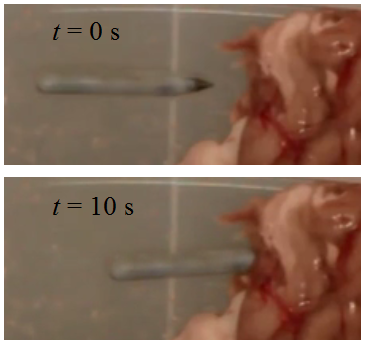
\includegraphics[width=150 pt]{tests_in_MRI.png}
  \caption{Picture of the magnetic hammer driven by an MRI scanner. The penetration test is realized on a sheep brain sample.}
  \label{MRI_test}
\end{figure}

\section{CONCLUSIONS}


\addtolength{\textheight}{-12cm}   % This command serves to balance the column lengths
                                  % on the last page of the document manually. It shortens
                                  % the textheight of the last page by a suitable amount.
                                  % This command does not take effect until the next page
                                  % so it should come on the page before the last. Make
                                  % sure that you do not shorten the textheight too much.

%%%%%%%%%%%%%%%%%%%%%%%%%%%%%%%%%%%%%%%%%%%%%%%%%%%%%%%%%%%%%%%%%%%%%%%%%%%%%%%%



%%%%%%%%%%%%%%%%%%%%%%%%%%%%%%%%%%%%%%%%%%%%%%%%%%%%%%%%%%%%%%%%%%%%%%%%%%%%%%%%

\bibliographystyle{unsrt}
\bibliography{biblio}



\end{document}